%%%%%%%%%%%%%%%%%%%%%%%%%%%%%%%%%%%%%%%%%%%%%%%%%%%%%%%%%%%%%%%%%%%%%%%
%                          template.tex
%
% LaTeX template for papers conforming to the United States Sections of
% the Combustion Institute style guide.
%
% Authors:
%     Bryan W. Weber, University of Connecticut
%     Kyle E. Niemeyer, Oregon State University
%
% This work is licensed under the Creative Commons Attribution 4.0
% International License. To view a copy of this license, visit
% http://creativecommons.org/licenses/by/4.0/.
%
% The source for this template can be found at
% https://github.com/pr-omethe-us/ussci-latex-template
%%%%%%%%%%%%%%%%%%%%%%%%%%%%%%%%%%%%%%%%%%%%%%%%%%%%%%%%%%%%%%%%%%%%%%%
\documentclass[12pt]{ussci}

% BibLaTeX and biber (not BibTeX) are used to process the references,
% so these packages must be installed on your system. All configuration
% for the bibliography and citations are done in the ussci.cls file
% Add your bibliography file here, replacing template.bib
\addbibresource{references.bib}
%======================================================================
% Replace "Reaction Kinetics" in the line below by your paper topic
\newcommand\papertopic{Combustion Theory and Modeling}

\usepackage{graphicx}

\usepackage[utf8]{inputenc}
\usepackage[T1]{fontenc}
\usepackage{csquotes}
\usepackage[english]{babel}

\usepackage{textcomp}
\usepackage{siunitx}
\usepackage[normalem]{ulem}

\usepackage{amsmath}
\usepackage{amssymb}
\usepackage[version=4]{mhchem}
\usepackage{subcaption}
\usepackage{booktabs}

% Diagram stuff
%\usepackage{tikz}
%\usetikzlibrary{shapes.geometric, arrows}


% Commonly used definitions
\def\cantera{\texttt{Cantera}}
\def\nreactions{\Phi}
\def\gasreactions{\tau}
\def\surfreactions{\theta}
\def\nspecies{\Psi}
\def\gasspecies{\lambda}
\def\surfspecies{\mu}
\def \bmh{5pt} %bmatrix height
\def \bmw{5pt} %bmatrix width
\newcommand{\pderv}[2]
{
    \frac{\partial #1}{\partial #2}
}
\newcommand{\jacsurfline}[1]
{
    \pderv{#1}{T} & \pderv{#1}{n_1} &
    \cdots & \pderv{#1}{n_\gasspecies}  & \pderv{#1}{s_{\gasspecies + 1}} &
    \cdots & \pderv{#1}{s_\surfspecies}\\[\bmh]
}
\newcommand{\dotsline}
{
    \vdots & \vdots &
    \ddots & \vdots & \vdots &
    \ddots & \vdots \\[\bmh]
}
\def\cantera{\texttt{Cantera}}
\def\sundials{\texttt{Sundials}}
\def\cvodes{\texttt{CVODES}}
\def\gmres{\texttt{GMRES}}
\def\spgmr{\texttt{SPGMR}}
\def\psolve{\texttt{PSolve}}
\def\eigen{\texttt{Eigen}}
\def\S{\mathcal{S}}
\def\C{\mathcal{C}}
\def\AP{\mathcal{P}}
\def\prodSpecies{\beta}
\def\reactSpecies{\alpha}
\newcommand{\F}[1]{\mathcal{F}(#1)}
\newcommand{\N}[2][]{\mathcal{N}^{#1}(#2)}
\newcommand{\J}[2][]{\mathcal{J}^{#1}(#2)}
\newcommand{\K}[2][]{\mathcal{K}^{#1}(#2)}
\newcommand{\R}[2][]{\mathcal{R}^{#1}(#2)}
\newcommand{\MP}[2][]{\mathcal{P}^{#1}(#2)}
\newcommand{\B}[2][]{\mathcal{B}^{#1}(#2)}
\DeclareSIUnit\concentration{\kilo\mole\per\meter\cubed}
\DeclareSIUnit\ratelaw{\kilo\mole\per\meter\cubed\per\second}
\DeclareSIUnit\mass{\kilo\gram}
\DeclareSIUnit\temperature{\kelvin}
\DeclareSIUnit\atm{atm}
\DeclareSIUnit\bar{bar}
\def\srate{\si{\kilo\mole\per\meter\squared\per\second}}

\title{Generalized preconditioning for accelerating the integration of reactors with coupled gas-surface chemistry}

\author[1]{Anthony S.~Walker}
\author[2]{Raymond L.~Speth}
\author[1,*]{Kyle E.~Niemeyer}

\affil[1]{School of Mechanical, Industrial, and Manufacturing Engineering, Oregon State University, Corvallis, OR, United States}
\affil[2]{Department of Aeronautics and Astronautics, Massachusetts Institute of Technology, Cambridge, MA, United States}

\begin{document}
\maketitle

\begin{abstract} % 100 to 300 words.
    Detailed modeling of combustion kinetics with practical applicability is prohibitively expensive due to the large size and stiffness of chemical kinetic models.
    Generalized preconditioning is a method that uses a semi-analytical Jacobian-based preconditioner and sparse linear algebra solvers to reduce the cost of integrating large kinetic models.
    In this study, we extend this preconditioning technique to more general-applications by including the capability of modeling surface chemistry.
    We tested this extension on a well-stirred reactor with surface chemistry.
    In this system, we use a combination of 11 different gas and a surface phase model to assess performance based on model size.
    These gas and surface combinations range from 69 species and 740 reactions to 1437 species and 8681 reactions.
    From these tests, we realized a range of speed-up from 1.1 to 533 for all of the tested models and determined some of the driving mechanisms behind the speed-up realized.
\end{abstract}

\begin{keyword}
Chemical kinetics\sep Implicit integrators\sep Sparse matrix\sep Preconditioner\sep Ordinary differential equations
\end{keyword}

\section{Introduction}

Phenomena involving reacting fluid flows play an important role in energy and transportation applications, but high-fidelity modeling of such problems can be prohibitively expensive.
Computational expense generally limits the number of reactions and species a model can have while maintaining practical applicability.
This limitation generally results in sacrificing detail in the application to reduce the expense of the model.
While methods like model reduction and hybrid chemistry have been effective~\cite{Lu2009, Pepiot2019}, they sacrifice detail in the simulation and ultimately can be limited when starting with extremely large and complicated models.
For example, models of secondary organic aerosols, volatile organic compounds, and methylalkenes have been developed in excess of 5000 species \cite{saunders1997world, li_modeling_2015, sarathy_comprehensive_2011}.
While model reduction can help, simulating these systems requires handling detailed models with large numbers of species and reactions to fully capture the evolution of these particular compounds.

Even with model reduction and hybrid chemistry, these large and costly models are still prohibitive.
In making modeling of expensive phenomena more tractable, we must also consider improvements to the integrators used.
These stiff systems of nonlinear ordinary differential equations (ODES) require implicit integration which can be very expensive due to the factorization of large matrices.
The number of operations scales cubically with system size for direct solutions of these systems making them impractical as model size grows.

% Paragraph about our study
In this study, we build on generalized preconditioning~\cite{walker2022generalized} to include surface chemistry.
Generalized preconditioning, built from Adaptive preconditioning~\cite{mcnenly_faster_2015}, uses a mole based semi-analytical Jacobian that makes several simplifications to accelerate its formulation.
Notably, the species-rate partial derivatives neglect third-body efficiencies and pressure dependence, and the temperature partial derivatives are approximated with finite differences.
Furthermore, the ``adaptive'' feature of the method prunes non-diagonal values when below a specified threshold to further increase sparsity.
We extend this to surface chemistry by including the contributions of surface species partial derivatives in the Jacobian.
We also apply the thresholding technique to the surface phase contributions in the same way as the gas phase contributions.
We implemented this within \cantera{}~\cite{cantera} to extend the capability of the sparse integration system to more complex cases.
We apply our extended method on a well-stirred reactor with surface chemistry and have the goal of obtaining large factors of speed up for more complicated cases which would make the method more practical in CFD and other types of simulations.


\section{Related Works}

This study expands on our previous work~\cite{walker2022generalized} and that of McNenly et al.~\cite{mcnenly_faster_2015}, which leverage preconditioning and system sparsity to speed up implicit integration.
The use of sparse integrators has been prevalent in solving systems of nonlinear and stiff ODEs for some time.
Integration nonlinear systems of ODEs generally relies on a suitable root-finding algorithm such as Newton's method; these, in turn, require solving some form of a linear system.
Similarly, solving the linear system associated with the nonlinear step has multiple approaches.
Consequently, there are multiple facets to these integrators, which can be focused on to improve the overall integration.

% Multigrid methods
The nonlinear portion of the solution to these systems has been approached from several angles.
CVODES uses a popular approach, relying on Newton's method for the nonlinear step with a variety of linear system solvers for the linear step~\cite{serban_cvodes_2003}.
Another class of similar approaches are Jacobian free Newton--Krylov methods, which are the same but avoid explicitly calculating the Jacobian matrix~\cite{knoll2004jacobian}.
Mulitgrid methods with full approximation scheme (FAS) are an alternative to Newton's method, using multiple grids and a nonlinear correction~\cite{henson2003multigrid}.
All these methods require solving a linear system of equations, and as such they may employ a preconditioned linear solver for their linear iterations.
Consequently, there has been extensive studies on both iterative and direct solutions to linear systems~\cite{hageman2012applied, duff2017direct}.

When solving the linear system for a nonlinear step, direct methods and iterative methods are the two primary approaches.
The most famous direct solution to linear systems is Gaussian elimination~\cite{grcar2011ordinary, higham2011gaussian}.
This has been studied from several angles and there are multiple strategies and algorithms for implementing it~\cite{trefethen1997numerical}.
There are other well-documented direct solutions to linear systems~\cite{heldring2007fast, duff2017direct} but they generally become prohibitively expensive for large systems~\cite{pearson2020preconditioners}.
In our application, we are dealing with relatively large systems of equations, making direct solutions intractable and consequently iterative methods are more relevant.

Among iterative methods, there are many different classical methods and algorithms that have been studied.
Conjugate gradient methods have been employed for decades to develop solutions to linear systems~\cite{chandra1978conjugate}.
Conjugate gradient methods have also been improved upon to develop methods like BiCGSTAB~\cite{van1992bi} and CSBCG~\cite{bank1994composite}.
The community continued to build on methods like BCG to develop QMR and similar algorithms\cite{freund1991qmr}.
All of these methods built upon the conjugate gradient ideology but there are other wide-spread classical approachs as well.

One of the most popular iterative algorithms for linear systems is generalized minimum residuals (GMRES) developed by Saad et al.~\cite{saad1986gmres}, which is what we use here.
Additionally, methods such as incomplete orthogonalization \cite{gear1983iterative}, matrix-free methods~\cite{brown1986matrix}, and reduced storage matrix methods~\cite{brown_reduced_1989} have been studied thoroughly.
There are many more classical iterative methods for developing solutions to linear systems such as Chebyshev iteration, Gauss-Seidel, successive over relaxation, and point Jacobi which are well documented~\cite{hageman1981applied, vorst1997linear, saad2003iterative}.

Classical algorithms and implementations aside, there are more recent developments in solutions to linear systems~\cite{tropp2010computational}.
Several two-step methods were developed for solving ill-conditioned linear systems~\cite{salkuyeh2011new, beik2018iterative} and semidefinite linear systems~\cite{salkuyeh2014iterative}.
A quasi-Chebyshev method was developed as an improved Chebyshev semi-iterative method~\cite{wen2013quasi}.
Similarly, an optimized version of SOR was developed \cite{meng2014practical}.
These solutions generally fall under the blanket of Krylov subspace methods, which often depend on or improve with the aide of a preconditioner \cite{benzi2002preconditioning, pearson2020preconditioners}.

Preconditioning a system can be largely problem-dependent and has been employed for quite some time~\cite{bramble1988preconditioning, trefethen1997numerical, chen2005matrix}.
Persson et al. studied the solution to compressible Navier--Stokes equations when applying preconditioned iterative methods and a discontinuous Galerkin spatial discretization\cite{persson_newton-gmres_2008}.
Liang et al.~\cite{liang_towards_2009} leveraged species-interaction sparsity in a proprietary integrator.
Anzt et al.~\cite{anzt_preconditioned_2017} considered graphics processing unit-based preconditioned iterative methods to leverage sparsity.
More recently, these strategies have been applied to combustion applications~\cite{marzouk_embedding_2012} and remain a popular method for improving performance.
McNenly et al. leveraged semi-analytical Jacobians in developing a method called adaptive preconditioning which they applied to resolve reactor systems~\cite{mcnenly_faster_2015}.
Lapointe et al.~\cite{lapointe_sparse_2019, lapointe_computationally-efficient_2020} resolved one-dimensional laminar flame simulations and flamelet calculations with adaptive preconditioning.
Most recently, Cheng et al. studied auto-ignition behavior of gasoline/ethanol blends and gasoline surrogates while applying adaptive preconditioning~\cite{cheng2020autoignition, cheng2021autoignition}.

Many of the aforementioned studies relay on some form of the Jacobian matrix as the preconditioner.
Consequently, the use of an analytical and semi-analytical Jacobians in solving these systems and forming preconditioners in lieu of expensive finite-difference Jacobians has become more prevalent as it can lead to performance improvements.
Perini et al.~\cite{perini_analytical_2012} developed a tool called \texttt{SpeedCHEM}, which applies exact and approximate analytical Jacobian formulations for gas kinetics that leverage sparsity.
They applied various integration strategies with these methods, including preconditioning and incomplete LU factorization~\cite{perini_study_2014}.
Perini et al.~\cite{perini_fast_2018} later sped up the integration of kinetic models using approximate exponential terms and logarithms.
Dijkmans et al.~\cite{dijkmans_gpu_2014} leveraged efficient routines on graphics processing units and an analytical Jacobian with in situ adaptive tabulation, coupled to accelerate simulations with detailed chemistry.
Similarly, Niemeyer et al.~\cite{niemeyer_pyjac_2017} developed an analytical Jacobian generator for chemical kinetics, \texttt{pyJac}, that improves performance over finite-differences.

Here, we extend generalized preconditioning to constant-volume reactors with coupled gas-phase and surface chemistry.
We analyze how these extensions impact performance of the solver and method.
We also seek to understand the fundamental reasons behind performance impacts based on tunable parameters and assumptions made.
We developed and tested multiple systems with these extensions to aid in filling these gaps in our knowledge.

\section{Methods}
\label{p1:methods-section}

\subsection{Surface Chemistry Jacobian}

We applied generalized preconditioning to a well-stirred reactor with surface chemistry included.
We provided a derivation and solution of the preconditioning method for ideal gas constant pressure in the previous paper \cite{walker2022generalized}, so here we focus on the development of the Jacobian terms for the surface chemistry reactions.
We specifically focus on the derivatives of individual species with respect to other species as the temperature derivatives are identical with the only difference being additional species in the summations.
We set up the system by defining a state vector of length $\ell = \surfspecies + \gasspecies + 1$, where $\surfspecies$ is the number of surface species and $\gasspecies$ is the number of gas phase species. 
The total number of species is represented as $\nspecies$.
Similarly, the number of gas phase reactions is $\gasreactions$, the number of surface phase reactions is $\surfreactions$, and the total number of reactions is $\nreactions$.

We represent this system with the state vector
\begin{equation}
    \S{} = \{T, n_1, n_2, n_3, \cdots, n_{\gasspecies}, n_{\gasspecies+1} \cdots, n_{\surfspecies}\},\quad\S{}\in\mathbb{R}^\ell \;,
\end{equation}
where $T$ is temperature, $n_{m}$ is the moles of species $m$ in either phase.
The Jacobian matrix used in this work is
\begin{equation}
    \J{\S{}} =
    \begin{bmatrix}
        \jacsurfline{\dot{T}}
        \jacsurfline{\dot{n}_{1}}
        \dotsline{}
        \jacsurfline{\dot{n}_{\gasspecies}}
        \jacsurfline{\dot{s}_{\gasspecies+1}}
        \dotsline{}
        \jacsurfline{\dot{s}_{\surfspecies}}
    \end{bmatrix} \;
\end{equation}
where some of the terms are approximated \cite{walker2022generalized}.

We want to model this system on a mole basis so that we may apply generalized preconditioning as was done in \cite{walker2022generalized}.
Since surface productions have units \si{\kilo\mole\per\meter\squared\per\second}, we multiply by the associated surface area.
Likewise, we multiply gas phase productions by the associated volume as they have units \si{\kilo\mole\per\meter\cubed\per\second}.
These conversions provide a molar rate for both phases in the system.
The mole-based species conservation equation for the $m^{th}$ species is
\begin{equation}
    \label{eq:species-cons}
    \frac{dn_{m}}{dt}\Big\vert_{gas} = V \dot{\omega}_{m} + A \dot{s}_{m},
\end{equation}
where $\dot{\omega}_{m}$ and $\dot{s}_{m}$ are the time rate of change of concentration of species $i$ for the gas and surface phases respectively \cite{walker2022generalized}.

The Jacobian requires that we develop the $\partial \dot{n}_{m}/\partial n_j$ terms.
We find these derivatives as
\begin{equation}
        \frac{\partial \dot{n}_{m}}{\partial n_j} = V\frac{\partial \dot{\omega}_{m}}{\partial n_j} + \frac{\partial V}{\partial n_j}\omega_{m}+ A\frac{\partial \dot{s}_{m}}{\partial n_j},
\end{equation}
for a constant pressure system with a surface and
\begin{equation}
    \frac{\partial \dot{n}_{m}}{\partial n_j} = V\frac{\partial \dot{\omega}_{m}}{\partial n_j} + A\frac{\partial \dot{s}_{m}}{\partial n_j},
\end{equation}
for a constant volume system with a surface.

The species production rates are typically found as products of concentrations raised to some power.
We must convert the derivatives of species production rates with respect to concentration into moles for both surface and gas phases.
The conversion of these derivatives requires the surface phase concentration, gas phase concentration, and the ideal gas law which are respectively
\begin{align}
    [n_i] &= \frac{n_i}{A},\label{eq:conc_surf}\\
    [n_i] &= \frac{n_i}{V}, \text{ and }\label{eq:conc_gas}\\
    P V &= N R T.\label{eq:ideal_gas}\\
\end{align}

We consider a generalized production rate $\dot{\gamma}_m$ where
\begin{equation}
    \dot{\gamma}_m = f(T, [n_1], \cdots, [n_\nspecies])
\end{equation}
and can represent either $\dot{\omega}_m$ or $\dot{s}_m$.
We can generalize the needed derivatives then by applying the chain rule
\begin{equation}
    \label{eq:gen_deriv}
    \frac{\partial \dot{\gamma}_m}{\partial n_j} = \frac{\partial \dot{\gamma}_m}{\partial T}\frac{\partial T}{\partial n_j} + \sum_{i=1}^{\nspecies}{\frac{\partial \dot{\gamma}_m}{\partial [n_i]}\frac{\partial[n_i]}{\partial n_j}}.
\end{equation}
which requires another chain rule expansion to obtain
\begin{equation}
    \frac{\partial T}{\partial n_j} = \sum_{i=1}^{\nspecies}{\frac{\partial T}{\partial [n_i]}\frac{\partial [n_i]}{\partial n_j}}.
\end{equation}
We then use Equations~\ref{eq:conc_surf},~\ref{eq:conc_gas}, and~\ref{eq:ideal_gas} to find the remaining derivatives.

We assume that the surface takes the temperature of the associated gas phase which
results in a simple expression when $n_j$ is a surface species,
\begin{equation}
    \frac{\partial \dot{\gamma}_m}{\partial n_j} =  \frac{1}{A}\frac{\partial \dot{\gamma}_m}{\partial [n_j]}.
\end{equation}
Similarly, when $n_j$ is a gas phase species constrained by the constant volume assumption, an equally simple result is found:
\begin{equation}
    \frac{\partial \dot{\gamma}_m}{\partial n_j} =  \frac{1}{V}\frac{\partial \dot{\gamma}_m}{\partial [n_j]}.
\end{equation}

When $n_j$ is a gas phase species constrained by the constant pressure assumption, the result becomes more complicated and we need to find all of the derivatives in Equation~\ref{eq:gen_deriv}.
We write temperature as a function of concentrations
\begin{equation}
    T = \frac{P}{R\sum_{i=1}^{\gasspecies}[n_i]}
\end{equation}
and use the constant pressure constraint to obtain
\begin{equation}
    \frac{\partial T}{\partial [n_i]} = -\frac{P}{R(\sum_{i=1}^{\gasspecies}[n_i])^{2}} = -\frac{P}{RC^{2}},
\end{equation}
where $C$ is the total molar concentration.
We can use the ideal gas law and definition of total molar concentration to obtain a simpler form of the former derivative as,
\begin{equation}
    \frac{\partial T}{\partial [n_i]}  = -\frac{P V^2}{N^2 R} = -\frac{VT}{N}.
\end{equation}
We now need to find $\partial [n_i] / \partial n_j$, so we write $[n_i]$ as a function of moles and temperature,
\begin{equation}
    [n_i] = \frac{P n_i}{R T \sum_{k=1}^{\gasspecies} n_k}.
\end{equation}
We generalize the derivative by introducing a kronecker delta,
\begin{equation}
    \delta_{ij} =
    \begin{cases}
            1, &         \text{if } i=j,\\
            0, &         \text{if } i\neq j.
    \end{cases}
\end{equation}
The needed derivatives are then
\begin{equation}
    \frac{\partial [n_i]}{\partial n_j} = \frac{P R T \delta_{i,j} \sum_{k=1}^{\gasspecies}{n_k} - P R T n_i}{(NRT)^2} = \frac{P(N\delta_{i,j}-n_i)}{N^2RT} = \frac{N\delta_{i,j}-n_i}{V N}.
\end{equation}
% where $X_i$ is the mole fraction of species $i$.

The development of the remaining derivatives with respect to concentration is straight forward as the production rates are a function of species concentrations.
We neglect rate coefficient coverage dependance here which makes the procedure identical for surface and gas phase species.
We can model $\dot{s}_{m}$ as
\begin{equation}
        \frac{d s_{m}}{dt} = \sum_{i=1}^{\surfreactions}{(\nu^{\prime\prime}_{k,i}-\nu^{\prime}_{k,i})q_i},\quad(k=1,...,\surfspecies)
\end{equation}
where $q_i$ is the rate of progress of for the $i^{th}$ reaction and $\nu^{\prime\prime}_{k,i}$ and $\nu^{\prime}_{k,i}$ are the stoichiometric coefficients for products and reactants of the $i^{th}$ reaction and $k^{th}$ species.
The rate of progress for the $i^{th}$ reaction is
\begin{equation}
        q_i = k_{f,i}\prod_{k=1}^{\nspecies}{s_k^{\nu^{\prime}_{k,i}}} - k_{r,i}\prod_{k=1}^{\nspecies}{s_k^{\nu^{\prime\prime}_{k,i}}}.
\end{equation}

We then obtain the derivative of $\dot{s}_m$ with respect to $[n_j]$ from the two former equations as
\begin{equation}
        \frac{\partial \dot{s}_{m}}{\partial [n_j]}  = \sum_{i=1}^{\surfreactions}{(\nu^{\prime\prime}_{k,i}-\nu^{\prime}_{k,i})\frac{\partial}{\partial s_j}\bigg(k_{f,i}\prod_{k=1}^{\nspecies}{s_k^{\nu^{\prime}_{k,i}}} - k_{r,i}\prod_{k=1}^{\nspecies}{s_k^{\nu^{\prime\prime}_{k,i}}}\bigg)}.
\end{equation}
We then finalize the derivative as
\begin{equation}
        \frac{\partial \dot{s}_{m}}{\partial [n_j]}  = \sum_{i=1}^{\surfreactions}{(\nu^{\prime\prime}_{k,i}-\nu^{\prime}_{k,i})\bigg(k_{f,i}\nu^\prime_{h,i}s_{m}^{\nu^\prime_{h,i}-1}\prod_{\substack{k = 1 \\ k \neq h}}^{\nspecies}{s_k^{\nu^{\prime}_{k,i}}} - k_{r,i}\nu^{\prime\prime}_{h,i}s_{m}^{\nu^{\prime\prime}_{h,i}-1}\prod_{\substack{k = 1 \\ k \neq h}}^{\nspecies}{s_k^{\nu^{\prime\prime}_{k,i}}}\bigg)}.
\end{equation}
The surface Jacobian contribution is then
\begin{equation}
    \label{surf_contrib}
    \frac{\partial \dot{n}_{m}}{\partial n_j}\Big\vert_{surface} = \sum_{i=1}^{\surfreactions}{(\nu^{\prime\prime}_{k,i}-\nu^{\prime}_{k,i})\bigg(k_{f,i}\nu^\prime_{h,i}s_{m}^{\nu^\prime_{h,i}-1}\prod_{\substack{k = 1 \\ k \neq h}}^{\nspecies}{s_k^{\nu^{\prime}_{k,i}}} - k_{r,i}\nu^{\prime\prime}_{h,i}s_{m}^{\nu^{\prime\prime}_{h,i}-1}\prod_{\substack{k = 1 \\ k \neq h}}^{\nspecies}{s_k^{\nu^{\prime\prime}_{k,i}}}\bigg)}
\end{equation}

The gas phase contributions are then described by
\begin{equation}
    \frac{\partial \dot{n}_{m}}{\partial n_j}\Big\vert_{gas} = V\frac{\partial \dot{\omega}_{m}}{\partial n_j} + \frac{\partial V}{\partial n_j}\omega_{m},
\end{equation}
which is thoroughly derived in \cite{walker2022generalized}.
The final expression for the gas phase contributions is
\begin{equation}
    \label{gas_contrib}
    \frac{\partial \dot{n}_{m}}{\partial n_j}\Big\vert_{gas} = \frac{V}{N}\dot{\omega}_{m} + \sum_{i=1}^{\gasreactions}{(\nu^{\prime\prime}_{k,i}-\nu^{\prime}_{k,i})\bigg(k_{f,i}\nu^\prime_{h,i}\omega_{m}^{\nu^\prime_{h,i}-1}\prod_{\substack{k = 1 \\ k \neq h}}^{\gasspecies}{\omega_k^{\nu^{\prime}_{k,i}}} - k_{r,i}\nu^{\prime\prime}_{h,i}\omega_{m}^{\nu^{\prime\prime}_{h,i}-1}\prod_{\substack{k = 1 \\ k \neq h}}^{\gasspecies}{\omega_k^{\nu^{\prime\prime}_{k,i}}}\bigg)}
\end{equation}

The overall contribution to the Jacobian is then
\begin{equation}
    \frac{\partial \dot{n}_{m}}{\partial n_j} = \frac{\partial \dot{n}_{m}}{\partial n_j}\Big\vert_{gas} + \frac{\partial \dot{n}_{m}}{\partial n_j}\Big\vert_{surface}
\end{equation}
where Equations~\eqref{surf_contrib} and~\eqref{gas_contrib} represent the contributions from each phase.

\subsection{Test Problems}
\label{sec:test-problems}

We implemented these equations in \cantera{} and tested the implementation with an ideal gas constant volume well-stirred reactor with surface chemistry.
We set up these problems with initial temperature and pressure conditions to produce an ignition event and integrated for one second in real time.
We ran all combinations of gas and surface models listed in Table~\ref{t1:mechanisms} to develop our results.
We ran each of these configurations 100 times on the computing cluster at Oregon State University and averaged the performance.
Figure~\ref{fig:wsr} shows how species evolve using the hydrogen model as an example to demonstrate the general behavior of each simulation.
We expect to see an equivalent drop in the reactants (e.g., \ce{H2}) with rise in products (e.g., \ce{H2O}), as seen in the figure.

\begin{figure}[htbp]
    \centering
    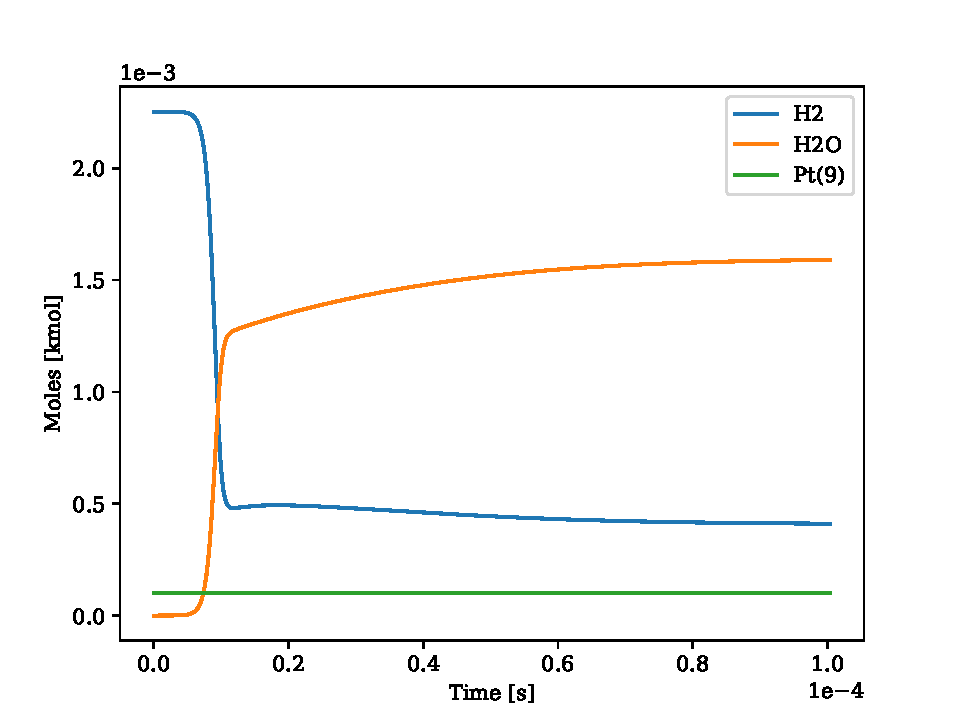
\includegraphics[scale=0.65]{figures/wsr_hydrogen.pdf}
    \caption{Selected species behavior for the well-stirred reactor over time.}
    \label{fig:wsr}
\end{figure}

Table~\ref{t1:mechanisms} lists the kinetics models used in this study with some basic information about each model.
We included 11 gas-phase models and one surface-phase model.
A complete test configuration for the well-stirred reactor would be a gas-phase model with the surface phase model.
Including both gas and surface phases, the smallest configuration has 69 species and 740 reactions and the largest has 1437 species and 8681 reactions.
All the models listed here and testing codes for the problems described are openly available on GitHub~\cite{testing_package}.

\begin{table}[htbp] \small
    \centering
    \begin{tabular}{@{}llll@{}}
        \toprule
        Model & Formula\slash fuel name(s) & Species & Reactions\\
        \midrule
        Hydrogen~\cite{smith_gri-mech_1999} & \ce{H2} & 10 & 29\\
        GRI-Mech 3.0~\cite{smith_gri-mech_1999} & \ce{CH4} & 55 & 325\\
        Platinum~\cite{kreitz2022detailed} & \ce{Pt} & 59 & 538\\
        DME-Propane~\cite{dames_detailed_2016} & \ce{CH3OCH3} \& \ce{C3H8} & 122 & 711\\
        HyChem Jet-A~\cite{wang_physics-based_2018, xu_physics-based_2018} & POSF 10325 (\ce{C11H22}) & 203 & 1589\\
        Butane~\cite{zhang_shock_2013} & \ce{C4H10} & 230 & 2461\\
        2-Butonane~\cite{hemken_2017} & \ce{C4H8O1}-2 & 315 & 1803\\
        Isobutene~\cite{li_2016} & \textit{i-}\ce{C4H8} & 493 & 2716\\
        \textit{n}-Heptane~\cite{mehl_kinetic_2011} & \textit{n-}\ce{C7H16} & 654 & 4846\\
        Isooctane~\cite{mehl_chemical_2009} & \textit{i-}\ce{C8H18} & 874 & 6864\\
        3-Methylheptane~\cite{mehl_chemical_2009} & \ce{C8H18}\ce{-3} & 1378 & 8143\\
        \bottomrule
    \end{tabular}
    \caption{Details on the chemical kinetic models used for testing.}
    \label{t1:mechanisms}
\end{table}

\section{Results \& discussion}

We extended generalized preconditioning to model gas-surface chemical interaction.
We ran the tests described in Section~\ref{sec:test-problems} to develop the figures in this section.
In Figure~\ref{fig:speed-up} we obtain a minimum speed up of 1.1 for hydrogen with platinum and a maximum of 533 for DME with platinum.
However, the behavior we see does not follow the trend of increasing speed-up with increasing numbers of species as found in past, gas-phase studies~\cite{walker2022generalized}.
We consequently look to other parameters of interest to understand why speed-up results deviate from what is expected.

\begin{figure}[htbp]
    \centering
    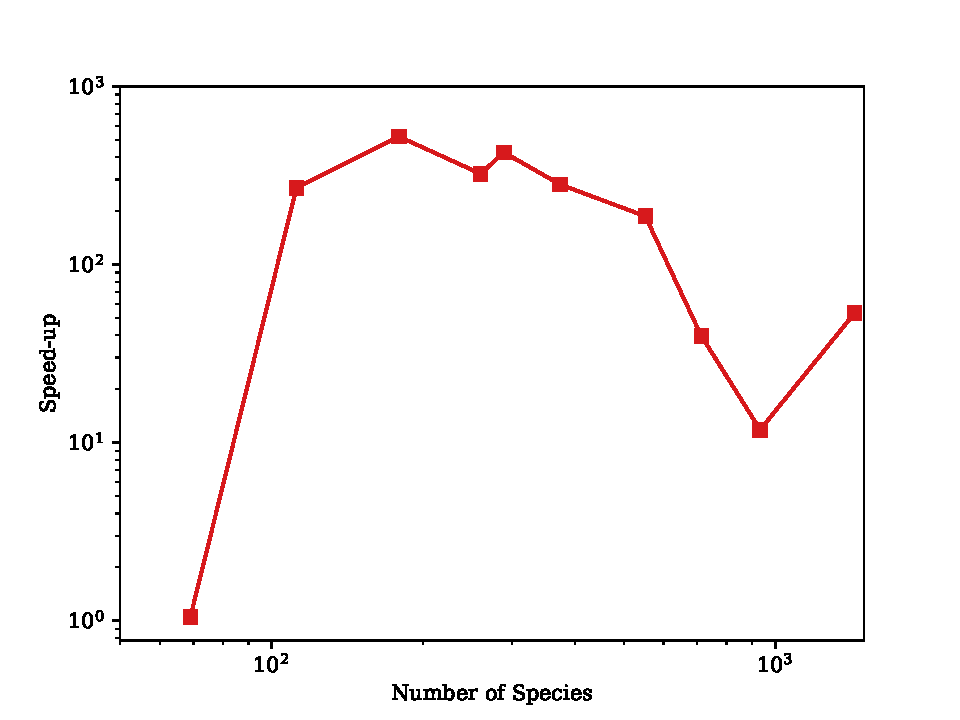
\includegraphics[scale=0.65]{figures/speed-up.pdf}
    \caption{Maximum speed-up obtained over a standard mass fraction integration.}
    \label{fig:speed-up}
\end{figure}

We first considered the number of nonlinear iterations as we can compare the nonlinear iterations of the preconditioned solver to that of the mass fraction based solver directly.
The ratio of nonlinear iterations for a standard integration to that of a preconditioned integration suggests the reduction of nonlinear iterations plays a role.
The trend of nonlinear iterations follows the speed-up directly with the exception of hydrogen and platinum.
While the trend is not as dramatic in Figure~\ref{fig:non-ratio} as it is in Figure~\ref{fig:speed-up}, it is influencing the speed-up.
The outlier in this case is likely due to a different bottleneck dominating the simulation with lower numbers of species and reactions.

\begin{figure}[htbp]
    \centering
    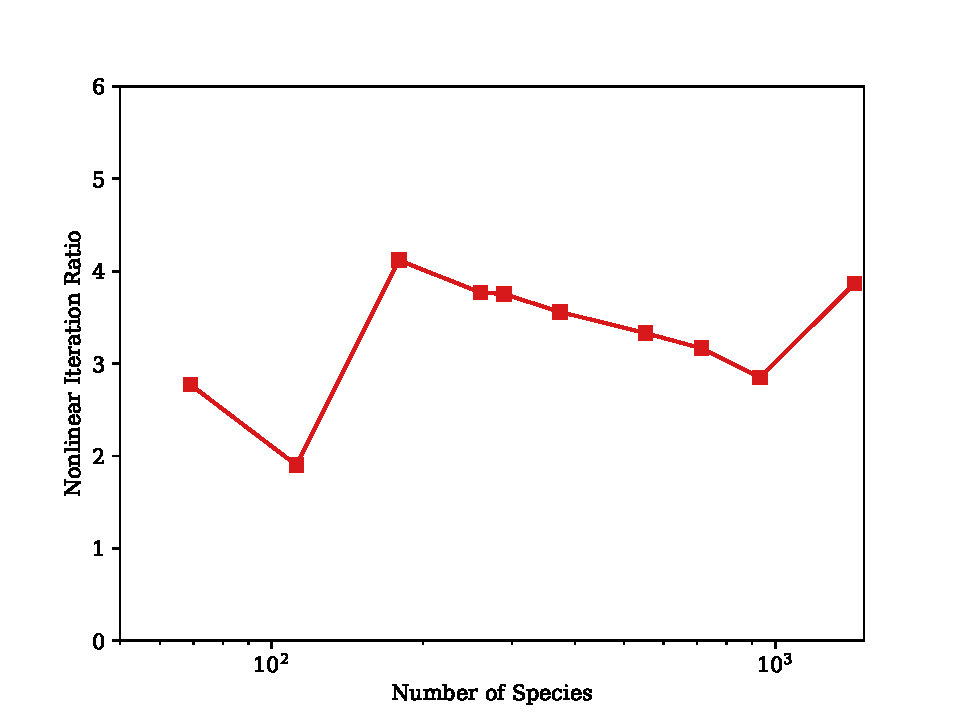
\includegraphics[scale=0.65]{figures/nonlinear_itrs.pdf}
    \caption{Ratio of nonlinear iterations for a standard integration to a preconditioned integration.}
    \label{fig:non-ratio}
\end{figure}

We further considered the linear iterations to explain the speed-up trend in Figure~\ref{fig:speed-up}. 
We expected an inverse relation between speed-up and linear iterations as was observed in~\cite{walker2022generalized}.
We see an inverse relation in Figure~\ref{fig:lin-iters} for models with greater numbers of species up than 2-butonane and platinum at 374 species. 
Otherwise, we see that the linear iterations track directly with the speed-up, which would suggest that there is yet another controlling factor.

\begin{figure}[htbp]
    \centering
    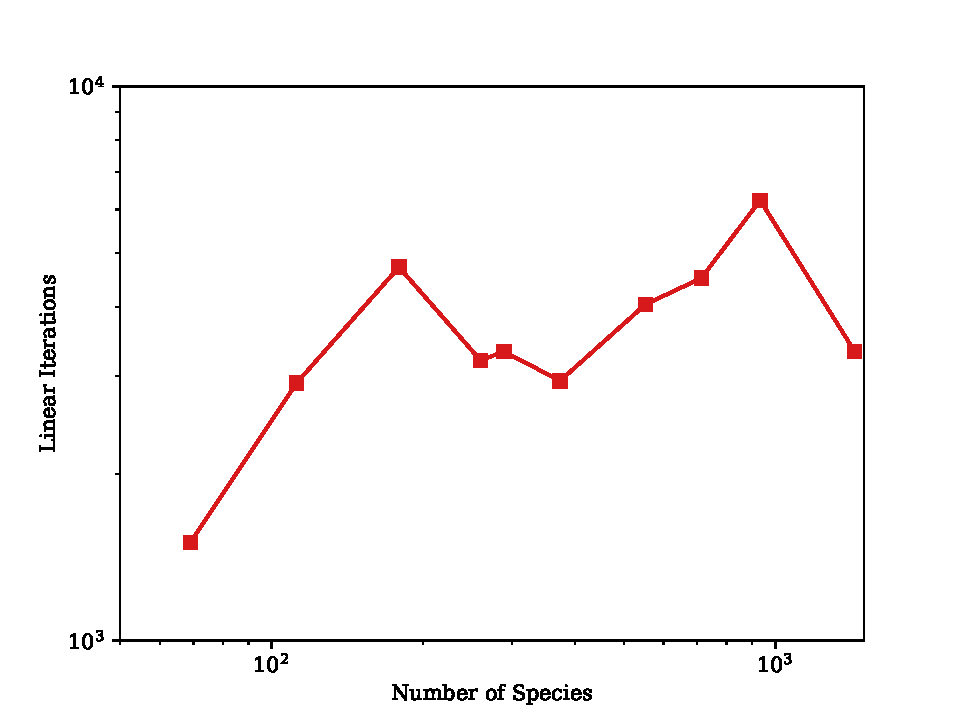
\includegraphics[scale=0.65]{figures/linear_itrs.pdf}
    \caption{Linear iterations of preconditioned integrations.}
    \label{fig:lin-iters}
\end{figure}

\section{Conclusions}

In conclusion, we tested a ideal-gas constant-volume well-stirred reactor with 11 gas phase models and a reacting surface. 
These gas and surface combinations range from 69 species and 740 reactions to 1437 species and 8681 reactions.
We realized a range of speed-up from 1.1 to 533 for all of the tested models which occur for hydrogen with platinum at 69 total species and DME with platinum at 179 total species respectively. 
The trend in speed-up however does not behave as initially expected based on former studies, which exhibit increasing speed-up with increasing numbers of species.

In the analyses so far, we have determined that reduction in nonlinear iterations tracks well with improved performance.
hydrogen with platinum is the only outlier in this regard and it is likely that the low number of species in this model is the cause.
However, this does not account for the large and unexpected variations in magnitude of the speed-up for the remaining models.
Similar to other studies, we have determined that the number of linear iterations plays a role in the performance but is not sole controlling factor and does not explain the drastic variation in magnitude.
The surface model in general has many species with zero values which likely contributes to spike in performance in models with fewer numbers of species as it bolsters the sparsity of the combined models.

Further study is need to better assess the newly introduced influence by adding surface chemistry to the preconditioned solver.
Consequently, our future work will consist of introducing more surface phase models and problem variation to determine if the speed-up trend is a result of this particular model and problem.
We also hope to further study the impact of assumptions and thresholding in the original gas-phase preconditioned solver.
We plan to assess the impact of assumptions by manipulating and comparing models with large compositions of reactions affected by the assumptions.
Finally, we plan to develop a better understand of performance improvements realized by thresholding and develop a basic heuristic for determining a threshold.

\section{Acknowledgements}
This material is based upon work supported by the National Science Foundation under Grant Nos.~1931592 (OSU) and 1931391 (MIT).

\printbibliography

\end{document}

% -------------------------------------------------------------------- %
% -------------------------------------------------------------------- %
% -------------------------------------------------------------------- %
